% Editable source for result.pdf, written by make_figures.py from run_github_38803625711/panel/result.json
\documentclass[tikz,border=6pt]{standalone}
\usepackage[T1]{fontenc}
\begin{document}
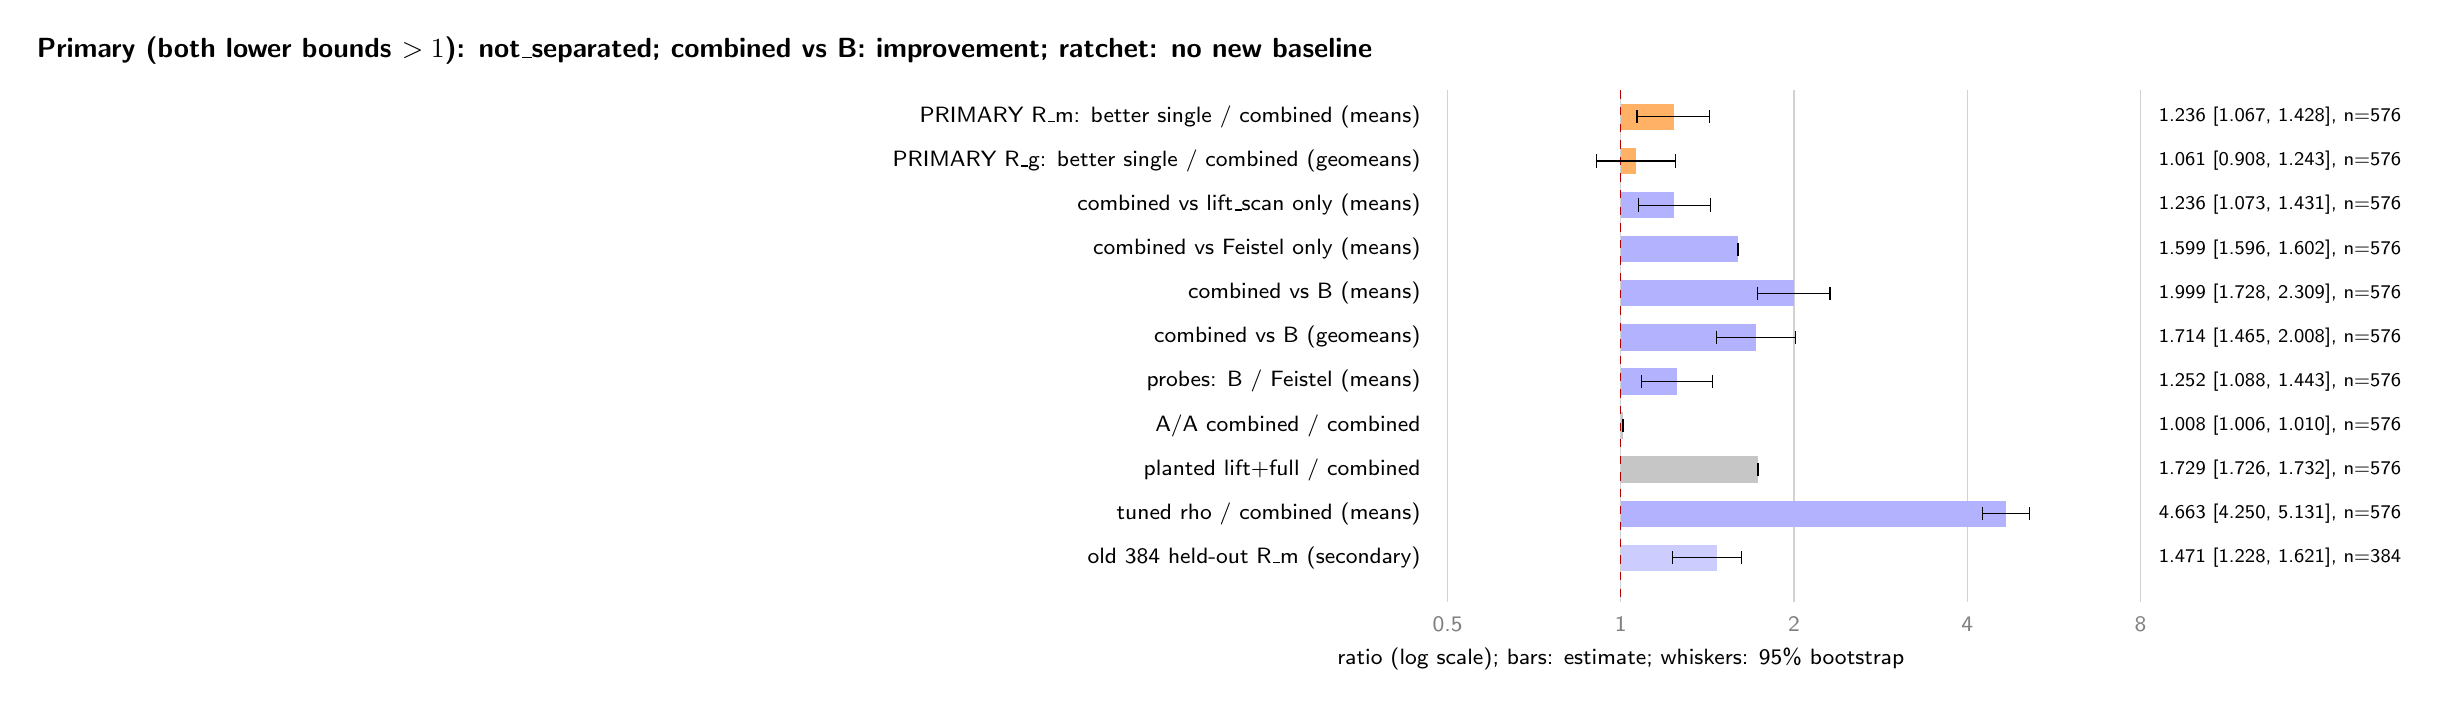
\begin{tikzpicture}[font=\sffamily\footnotesize,x=22mm,y=-5.6mm]
\draw[gray!35] (-1.0000,-0.6) -- (-1.0000,11); \node[gray] at (-1.0000,11.5) {0.5};
\draw[gray!35] (0.0000,-0.6) -- (0.0000,11); \node[gray] at (0.0000,11.5) {1};
\draw[gray!35] (1.0000,-0.6) -- (1.0000,11); \node[gray] at (1.0000,11.5) {2};
\draw[gray!35] (2.0000,-0.6) -- (2.0000,11); \node[gray] at (2.0000,11.5) {4};
\draw[gray!35] (3.0000,-0.6) -- (3.0000,11); \node[gray] at (3.0000,11.5) {8};
\draw[red!70!black,dashed] (0,-0.6) -- (0,11);
\node at (0,12.3) {ratio (log scale); bars: estimate; whiskers: 95\% bootstrap};
\node[anchor=west,font=\sffamily\bfseries] at (-9.2,-1.5) {Primary (both lower bounds $>1$): not\_separated; combined vs B: improvement; ratchet: no new baseline};
\node[anchor=east] at (-1.1000,0) {PRIMARY R\_m: better single / combined (means)};
\fill[orange!60] (0,-0.300000) rectangle (0.3060,0.300000);
\draw (0.0937,0) -- (0.5136,0); \draw (0.0937,-0.150000) -- (0.0937,0.150000); \draw (0.5136,-0.150000) -- (0.5136,0.150000);
\node[anchor=west,font=\sffamily\scriptsize] at (3.0500,0) {1.236 [1.067, 1.428], n=576};
\node[anchor=east] at (-1.1000,1) {PRIMARY R\_g: better single / combined (geomeans)};
\fill[orange!60] (0,0.700000) rectangle (0.0856,1.300000);
\draw (-0.1387,1) -- (0.3139,1); \draw (-0.1387,0.850000) -- (-0.1387,1.150000); \draw (0.3139,0.850000) -- (0.3139,1.150000);
\node[anchor=west,font=\sffamily\scriptsize] at (3.0500,1) {1.061 [0.908, 1.243], n=576};
\node[anchor=east] at (-1.1000,2) {combined vs lift\_scan only (means)};
\fill[blue!30] (0,1.700000) rectangle (0.3060,2.300000);
\draw (0.1021,2) -- (0.5167,2); \draw (0.1021,1.850000) -- (0.1021,2.150000); \draw (0.5167,1.850000) -- (0.5167,2.150000);
\node[anchor=west,font=\sffamily\scriptsize] at (3.0500,2) {1.236 [1.073, 1.431], n=576};
\node[anchor=east] at (-1.1000,3) {combined vs Feistel only (means)};
\fill[blue!30] (0,2.700000) rectangle (0.6775,3.300000);
\draw (0.6749,3) -- (0.6801,3); \draw (0.6749,2.850000) -- (0.6749,3.150000); \draw (0.6801,2.850000) -- (0.6801,3.150000);
\node[anchor=west,font=\sffamily\scriptsize] at (3.0500,3) {1.599 [1.596, 1.602], n=576};
\node[anchor=east] at (-1.1000,4) {combined vs B (means)};
\fill[blue!30] (0,3.700000) rectangle (0.9994,4.300000);
\draw (0.7895,4) -- (1.2073,4); \draw (0.7895,3.850000) -- (0.7895,4.150000); \draw (1.2073,3.850000) -- (1.2073,4.150000);
\node[anchor=west,font=\sffamily\scriptsize] at (3.0500,4) {1.999 [1.728, 2.309], n=576};
\node[anchor=east] at (-1.1000,5) {combined vs B (geomeans)};
\fill[blue!30] (0,4.700000) rectangle (0.7776,5.300000);
\draw (0.5506,5) -- (1.0058,5); \draw (0.5506,4.850000) -- (0.5506,5.150000); \draw (1.0058,4.850000) -- (1.0058,5.150000);
\node[anchor=west,font=\sffamily\scriptsize] at (3.0500,5) {1.714 [1.465, 2.008], n=576};
\node[anchor=east] at (-1.1000,6) {probes: B / Feistel (means)};
\fill[blue!30] (0,5.700000) rectangle (0.3246,6.300000);
\draw (0.1213,6) -- (0.5291,6); \draw (0.1213,5.850000) -- (0.1213,6.150000); \draw (0.5291,5.850000) -- (0.5291,6.150000);
\node[anchor=west,font=\sffamily\scriptsize] at (3.0500,6) {1.252 [1.088, 1.443], n=576};
\node[anchor=east] at (-1.1000,7) {A/A combined / combined};
\fill[gray!45] (0,6.700000) rectangle (0.0116,7.300000);
\draw (0.0084,7) -- (0.0149,7); \draw (0.0084,6.850000) -- (0.0084,7.150000); \draw (0.0149,6.850000) -- (0.0149,7.150000);
\node[anchor=west,font=\sffamily\scriptsize] at (3.0500,7) {1.008 [1.006, 1.010], n=576};
\node[anchor=east] at (-1.1000,8) {planted lift+full / combined};
\fill[gray!45] (0,7.700000) rectangle (0.7899,8.300000);
\draw (0.7871,8) -- (0.7926,8); \draw (0.7871,7.850000) -- (0.7871,8.150000); \draw (0.7926,7.850000) -- (0.7926,8.150000);
\node[anchor=west,font=\sffamily\scriptsize] at (3.0500,8) {1.729 [1.726, 1.732], n=576};
\node[anchor=east] at (-1.1000,9) {tuned rho / combined (means)};
\fill[blue!30] (0,8.700000) rectangle (2.2212,9.300000);
\draw (2.0875,9) -- (2.3592,9); \draw (2.0875,8.850000) -- (2.0875,9.150000); \draw (2.3592,8.850000) -- (2.3592,9.150000);
\node[anchor=west,font=\sffamily\scriptsize] at (3.0500,9) {4.663 [4.250, 5.131], n=576};
\node[anchor=east] at (-1.1000,10) {old 384 held-out R\_m (secondary)};
\fill[blue!20] (0,9.700000) rectangle (0.5568,10.300000);
\draw (0.2967,10) -- (0.6971,10); \draw (0.2967,9.850000) -- (0.2967,10.150000); \draw (0.6971,9.850000) -- (0.6971,10.150000);
\node[anchor=west,font=\sffamily\scriptsize] at (3.0500,10) {1.471 [1.228, 1.621], n=384};
\end{tikzpicture}
\end{document}
